% =============================================================================
%  Plantilla de tesis / trabajo de grado - Universidad Pontificia Bolivariana
%  Clase upbthesis v3.0 (formato APA 7)
%
%  Compilación (requiere biber + biblatex-apa, ver README.md):
%     pdflatex upbthesis
%     biber    upbthesis
%     pdflatex upbthesis
%     pdflatex upbthesis
%  o, más cómodo:  latexmk -pdf upbthesis.tex
% =============================================================================

% Opciones de la clase:
%   Tamaño de fuente .... 10pt | 11pt | 12pt        (def. 12pt)
%   Caras ............... oneside | twoside          (def. oneside)
%   Interlineado ........ singlespace | onehalfspace | doublespace (def. onehalfspace)
%   Formato/citas ....... apa  (APA 7, recomendado) | numcit (Vancouver) | icontec
%   Idioma .............. spanish | english          (def. spanish)
%   Impresión ........... print  (márgenes simétricos para imprimir)
\documentclass[12pt,oneside,onehalfspace,apa,spanish]{upbthesis}

% --- Paquetes adicionales del documento (opcionales) -------------------------
\usepackage{amsmath,amssymb}   % matemáticas, si las necesita
\usepackage{tabularx}          % tablas de ancho fijo (p. ej. la lista de siglas)

% --- Fuente bibliográfica (formato APA 7 vía biblatex) -----------------------
\addbibresource{upbthesis.bib}

% --- Datos de la portada -----------------------------------------------------
\title{Título del Trabajo de Grado: Subtítulo Descriptivo si Aplica}
\author{Nombre y Apellidos del Autor}
\school{Escuela de Ingenierías}
\faculty{Maestría en Ingeniería}
\address{Medellín, Antioquia, Colombia}
\degree{Trabajo de grado de maestría presentado para optar al título de Magíster en Ingeniería}
\director{Nombre del Director, Doctor (PhD) en Ingeniería}
\logo{img/logo-upb.png}        % opcional; este es el valor por defecto

% --- hyperref SIEMPRE al final del preámbulo ---------------------------------
\usepackage[colorlinks=true,linkcolor=black,citecolor=black,urlcolor=black]{hyperref}

\begin{document}

% =====================  PRELIMINARES  =======================================
\frontmatter

\maketitle          % Portada con logo (1 página en modo apa)
\originality        % Declaración de originalidad (texto reglamentario UPB)

\begin{dedication}
[Escriba aquí la dedicatoria. Es opcional.]
\end{dedication}

\begin{acknowledgements}
Texto de agradecimientos centrado.
\end{acknowledgements}

\begin{resumen}
[Resumen en español, máximo 250 palabras y en un solo párrafo. Plantee el
contexto del problema, el objetivo del trabajo, la metodología empleada, los
principales resultados y la conclusión más relevante.]
\end{resumen}
\begin{pclave}
Palabra clave 1; palabra clave 2; palabra clave 3; palabra clave 4.
\end{pclave}

\begin{abstract}
[English abstract, up to 250 words in a single paragraph, equivalent to the
Spanish resumen above.]
\end{abstract}
\begin{keywords}
Keyword 1; keyword 2; keyword 3; keyword 4.
\end{keywords}

\tableofcontents
\listoftables
\listoffigures

\begin{siglas}
\noindent
\begin{tabularx}{\textwidth}{l X}
  \textbf{APA}     & American Psychological Association \\
  \textbf{Cms.}    & Centímetros \\
  \textbf{ERIC}    & Education Resources Information Center \\
  \textbf{Esp.}    & Especialista \\
  \textbf{MP}      & Magistrado Ponente \\
  \textbf{MSc}     & Magister Scientiae \\
  \textbf{Párr.}   & Párrafo \\
  \textbf{PhD}     & Philosophiae Doctor \\
  \textbf{PBQ-SF}  & Personality Belief Questionnaire Short Form \\
  \textbf{PostDoc} & PostDoctor \\
  \textbf{UPB}     & Universidad Pontificia Bolivariana \\
\end{tabularx}
\end{siglas}

\begin{gloss}
TÉRMINO 1: definición breve del término.

TÉRMINO 2: definición breve del término.
\end{gloss}

% =====================  CUERPO DEL DOCUMENTO  ===============================
\mainmatter

\begin{introduction}
La introducción presenta el tema, su relevancia y la organización del documento.
Para citar dentro del texto en formato APA se usan dos comandos de biblatex:
la cita entre paréntesis \parencite{perez2021} y la cita narrativa, en la que
el autor forma parte de la oración, como en \textcite{rodriguez2022}. También
pueden citarse recursos en línea \parencite{lopez2023}.
\end{introduction}

\chapter{Marco teórico}
Texto introductorio del capítulo. Observe que el título del capítulo aparece
centrado, en negrita, con el formato «\textit{número.\ título}» y sin la
palabra «Capítulo», conforme al estilo APA 7.

\section{Primera sección}
Texto de la primera sección. Las secciones (nivel 1) van en negrita.

\section{Segunda sección}
Texto de la segunda sección, que a su vez contiene subdivisiones.

\subsection{Una subsección}
Las subsecciones (nivel 2) van en negrita y cursiva.

\subsubsection{Una subsubsección}
Las subsubsecciones (nivel 3) van en negrita.

% ---------------------------- Ejemplo de TABLA 1 ----------------------------
\begin{table}[htbp]
  \caption{Comparación de indicadores por categoría}
  \label{tab:indicadores}
  \centering
  \begin{tabular}{lcc}
    \toprule
    Categoría & Indicador A & Indicador B \\
    \midrule
    Grupo 1 & 0,82 & 0,71 \\
    Grupo 2 & 0,65 & 0,58 \\
    Grupo 3 & 0,90 & 0,84 \\
    \bottomrule
  \end{tabular}

  \smallskip
  {\footnotesize \textit{Nota.} Valores normalizados en el rango [0, 1].
   Elaboración propia.}
\end{table}

Como se observa en la Tabla~\ref{tab:indicadores}, el Grupo~3 presenta los
valores más altos en ambos indicadores. Note que el rótulo «Tabla 1» va en
negrita en su propia línea y el título en cursiva, encima de la tabla.

\chapter{Metodología y resultados}

\section{Procedimiento}
Descripción del procedimiento. A continuación se incluye una figura de ejemplo.

% --------------------------- Ejemplo de FIGURA 1 ----------------------------
\begin{figure}[htbp]
  \caption{Curva de codo para la selección del número de grupos}
  \label{fig:codo}
  \centering
  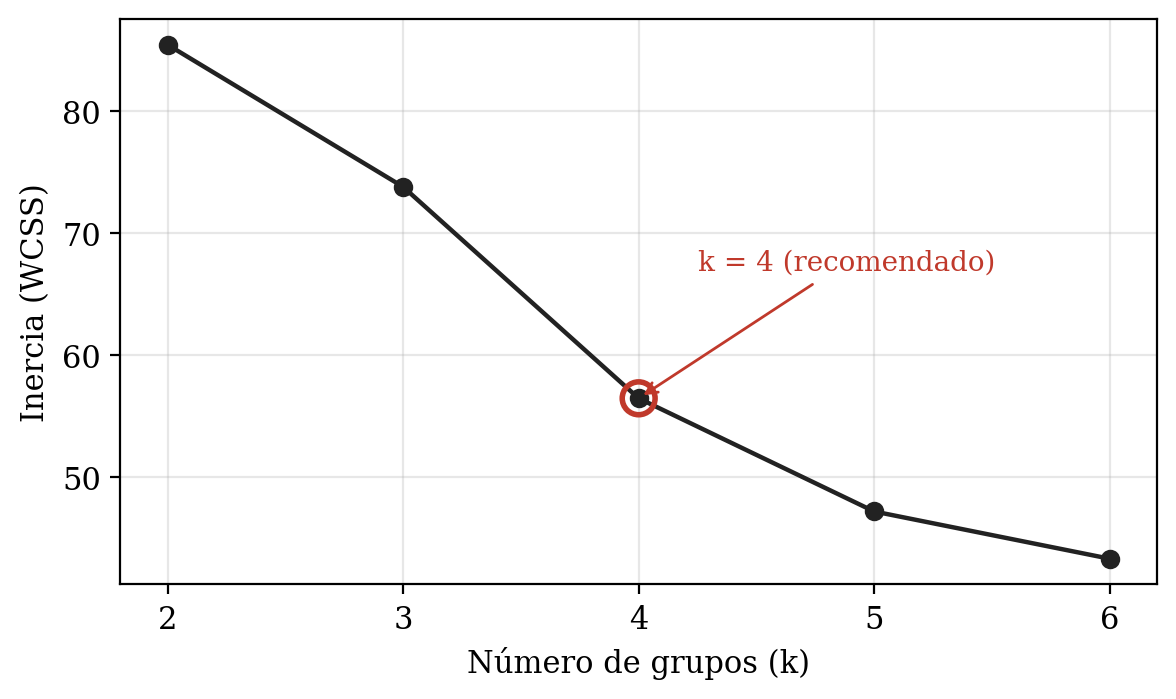
\includegraphics[width=0.7\textwidth]{img/ejemplo-figura1.png}

  \smallskip
  {\footnotesize \textit{Nota.} El «codo» sugiere el valor adecuado de $k$.
   Elaboración propia.}
\end{figure}

La Figura~\ref{fig:codo} muestra cómo se selecciona el número de grupos. El
rótulo de la figura también va arriba, en el mismo estilo que las tablas.

\section{Resultados}
Presentación de los resultados, apoyada en una segunda tabla y una segunda figura.

% ---------------------------- Ejemplo de TABLA 2 ----------------------------
\begin{table}[htbp]
  \caption{Resumen de métricas del modelo}
  \label{tab:metricas}
  \centering
  \begin{tabular}{lc}
    \toprule
    Métrica & Valor \\
    \midrule
    Precisión & 0,91 \\
    Exhaustividad & 0,88 \\
    Medida F1 & 0,89 \\
    \bottomrule
  \end{tabular}

  \smallskip
  {\footnotesize \textit{Nota.} Resultados sobre el conjunto de prueba.}
\end{table}

Las tablas y figuras se numeran de forma consecutiva en todo el documento
(Tabla~\ref{tab:metricas} y Figura~\ref{fig:codo}), no por capítulo, como
indica APA 7.

\chapter{Conclusiones}
Síntesis de los hallazgos y su relación con los objetivos del trabajo.

% =====================  REFERENCIAS  ========================================
\printbibliography[heading=bibintoc,title={Referencias}]

\end{document}
